\documentclass{siamart1116}
\usepackage{amsmath, amssymb}
%\usepackage{amsmath,amssymb,amsfonts,graphicx,amsthm,dsfont}
%\usepackage{listings}
%\usepackage{courier}
\usepackage{enumerate}
%\usepackage{color}
%\usepackage[usenames,dvipsnames]{xcolor}
%\usepackage{hyperref,tikz,mdframed}
%\hypersetup{colorlinks=true,urlcolor=MidnightBlue,citecolor=PineGreen,linkcolor=BrickRed}

% \lstset{
% 	basicstyle=\small\ttfamily,
% 	keywordstyle=\color{blue},
% 	language=python,
% 	xleftmargin=16pt,
% }
\usepackage{algorithmicx}
\usepackage{algpseudocode}% http://ctan.org/pkg/algorithmicx
\usepackage{multicol}

\textwidth=5.8in
\textheight=9in
\topmargin=-0.5in
\headheight=0in
\headsep=.5in
\hoffset  -.4in
\pagestyle{empty}

\newcommand{\Fp}{\mathbb{F}_p}
\newcommand{\Q}{\mathbb{Q}}
\newcommand{\Z}{\mathbb{Z}}
\newcommand{\kron}[2]{\left(\frac{#1}{#2}\right)}
\newcommand{\Aut}{\mathrm{Aut}}
\newcommand{\End}{\mathrm{End}}
\newcommand{\SO}{\mathrm{SO}}
\newcommand{\SU}{\mathrm{SU}}
\newcommand{\tr}{\operatorname{tr}}
\newcommand{\dee}{\mathrm{d}}
\newcommand{\deee}{\textbf{\text{\emph{d}}}}

\newcommand{\md}[1]{\textcolor{cyan}{#1}}

\newcommand{\TheAuthors}{V. Chen}

%\newtheorem{theorem}{Theorem}
%\newtheorem{definition}{Definition}

\graphicspath{ {graphics/} }

\title{Week 1 Summary}
\author{\TheAuthors}
\date{}
\begin{document}
\maketitle
\setlength{\unitlength}{1in}
\setlength{\parindent}{0in}


\section{Nonzero gamma}
I finished implementing the model that handles nonzero $\gamma$ in the likelihood. I ran some experiments using this algorithm on the voting records data set: $\beta = 0.9$ allowed for an acceptance probability of around $40\%$, and $\gamma = 1$ correctly classified around $87\%$ of the unlabeled senators. See \cref{fig:gamma_fig}, \cref{fig:gamma_prob}. The full parameters of the run are as follows:

\begin{center}
\begin{tabular}{| c | c |}
\hline
Iterations & 10000 \\ \hline
Burn in period & 5000 \\ \hline
Weight function parameters $(p, q, l)$ & $(2,2,1)$ \\ \hline
$\beta$ & $0.9$\\ \hline
$\gamma$ & $1$\\ \hline
$\tau$ & $0$\\ \hline
$\alpha$ & $1$\\ \hline
Labeled +1 & $280, 281, 282, 283$ \\ \hline
Labeled -1 & $25, 26, 27, 28$ \\ \hline
Percent of correct classification & $0.868852$ \\ \hline
\end{tabular}
\end{center}
\begin{figure}[htbp]
    \centering
    \label{fig:gamma_fig}
    \caption{Average of sign sample vector post burn-in period}
    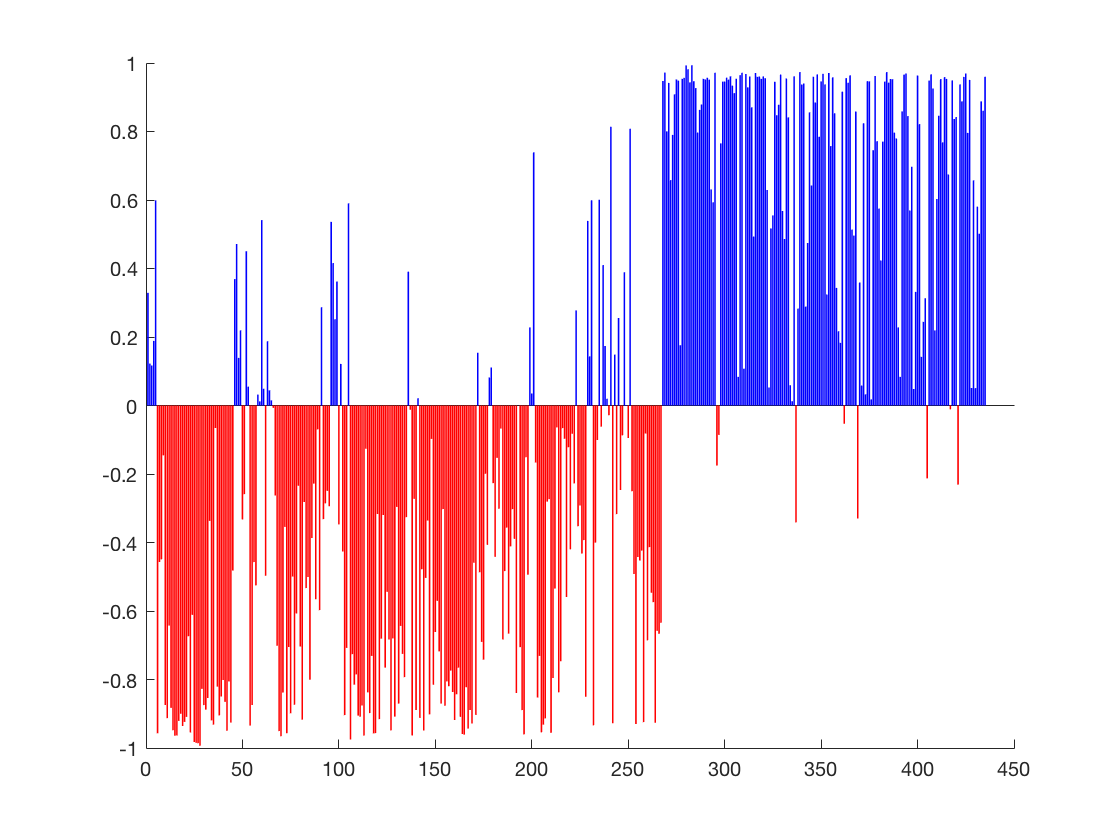
\includegraphics[width=.5\linewidth]{gamma_avg.png}
\end{figure}
\begin{figure}[htbp]
    \centering
    \label{fig:gamma_prob}
    \caption{Running average of MCMC acceptance probability post burn-in period}
    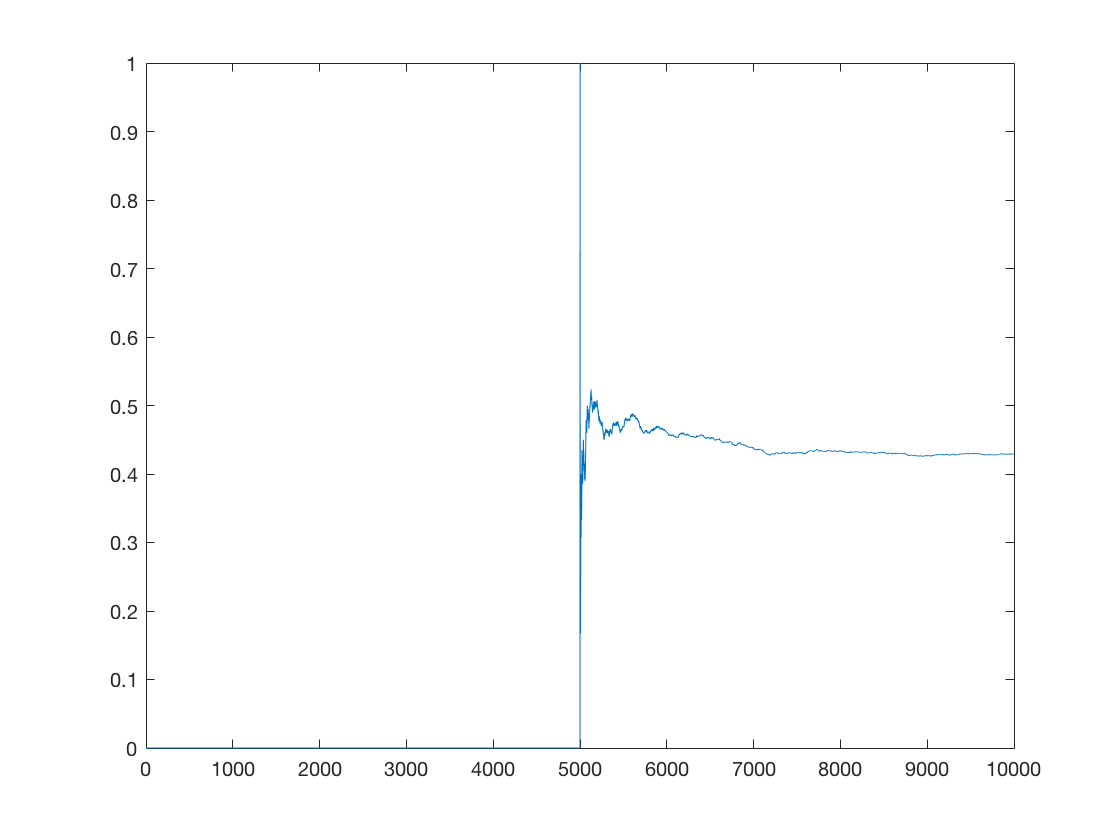
\includegraphics[width=.5\linewidth]{gamma_probability.png}
\end{figure}

\section{Learning $\tau, \alpha$}
I implemented \cref{alg:hierarchical_tau_alpha}, a hierarchical algorithm on $\tau$ and $\alpha$.
\begin{algorithm}
\caption{Hierarchical on $\tau, \alpha$}
\label{alg:hierarchical_tau_alpha}
\begin{algorithmic}
\State Initialize $\mu^{(0)} = (0, 1, 0, 0, \ldots)$, which is the Fiedler vector written in the orthonormal basis of the eigenvectors
\State Initialize $u^{(0)}$ as $\mu^{(0)}$ expressed in the standard basis.
\State Initialize $\tau^{(0)}, \alpha^{(0)}$. Select $\beta \in [0, 1]$
\State Initialize $\epsilon$
\For{$i = 0$ to $n$}
\State Sample $\xi$ from the prior distribution and expressed in the eigenbasis \Comment{$u|y, \tau, \alpha$}
\State Set a proposal $\nu^{(i)} = (1- \beta^2)^{1/2}\mu^{(i)} + \beta \xi$
\State Compute $v^{(i)}$ as $\nu^{(i)}$ in the standard basis
\State Set $u^{(i+1)} = v^{(i)}$ and $\mu^{(i+1)} = \nu^{(i)}$ with probability $\min (1, \exp(\Phi(u^{(i)}) - \Phi(v^{(i)})) )$

\State Set a proposal $t^{(i)} = \tau^{(i)} + \epsilon \zeta^{(i)}$ for $\zeta^{(i)} \sim N(0, 1)$ \Comment{$\tau|y,u,\alpha$}
\State Set $\tau^{(i+1)} = t^{(i)}$ with probability given by the ratio between the joint posterior functions on $u, \tau, \alpha$: $f(\mu^{(i+1)}, t^{(i)}, \alpha^{(i)})/f(\mu^{(i+1)}, \tau^{(i)}, \alpha^{(i)})$ (using the eigenbasis representation to simplify computation)

\State Set a proposal $a^{(i)} = \alpha^{(i)} + \epsilon \zeta^{(i)}$ for $\zeta^{(i)} \sim N(0, 1)$ \Comment{$\alpha|y,u,\tau$}
\State Set $\alpha^{(i+1)} = a^{(i)}$ with probability given by $f(\mu^{(i+1)}, \tau^{(i+1)}, a^{(i)})/f(\mu^{(i+1)}, \tau^{(i+1)}, \alpha^{(i)})$
\EndFor\\
\Return $u, \tau, \alpha$
\end{algorithmic}
\end{algorithm}

I additionally restricted the proposals for $\tau \in [0, 1]$ and $\alpha \in [0, 10]$. The results do not indicate that the MCMC is converging on a value for $\tau, \alpha$ at 100000 iterations, so maybe there is a bug in the algorithm or the code. Some of the gathered results follow. The parameters omitted in the following tables have the same values as in the nonzero gamma MCMC.

\begin{center}
\begin{tabular}{| c | c |}
\hline
Iterations & 100000 \\ \hline
Burn in period & 50000 \\ \hline
$\epsilon$ & $0.1$\\ \hline
Initial $\tau$ & $0$\\ \hline
Initial $\alpha$ & $1$\\ \hline
Average $\tau$ & $0.304877$\\ \hline
Average $\alpha$ & $7.014584$\\ \hline
Percent of correct classification & $0.871194$ \\ \hline
Time elapsed & 918.02 s \\ \hline
\end{tabular}
\end{center}

\begin{center}
\begin{tabular}{| c | c |}
\hline
Iterations & 100000 \\ \hline
Burn in period & 50000 \\ \hline
$\epsilon$ & $0.1$\\ \hline
Initial $\tau$ & $0.5$\\ \hline
Initial $\alpha$ & $0.5$\\ \hline
Average $\tau$ & $0.154294$\\ \hline
Average $\alpha$ & $2.960191$\\ \hline
Percent of correct classification & $0.868852$ \\ \hline
Time elapsed & 925.47 s \\ \hline
\end{tabular}
\end{center}

\begin{figure}[!htb]
    \begin{minipage}{0.48\textwidth}
        \centering
        \caption{$\tau^{(0)} = 0, \alpha^{(0)} = 1$, $\tau$ acceptance probability}
        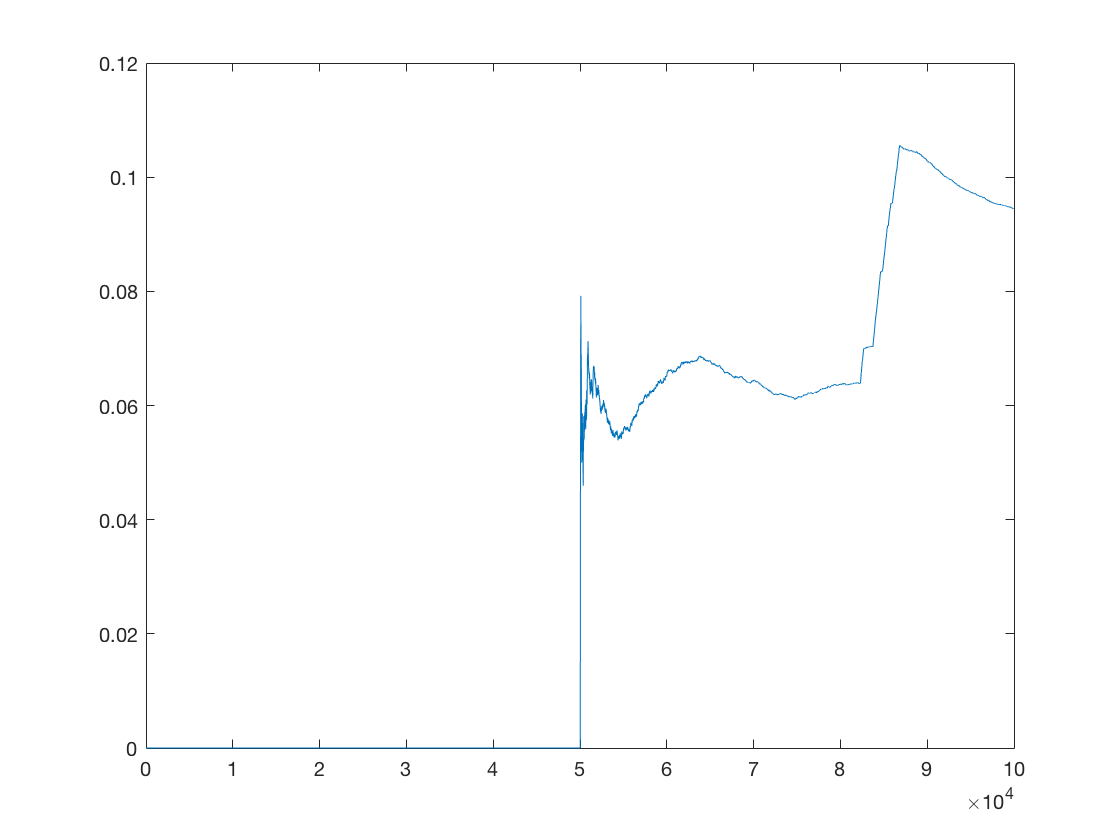
\includegraphics[width=\linewidth]{zero_one_tau_prob.png}
    \end{minipage} \hfill
    \begin{minipage}{0.48\textwidth}
        \centering
        \caption{$\tau^{(0)} = 0.5, \alpha^{(0)} = 0.5$, $\tau$ acceptance probability}
        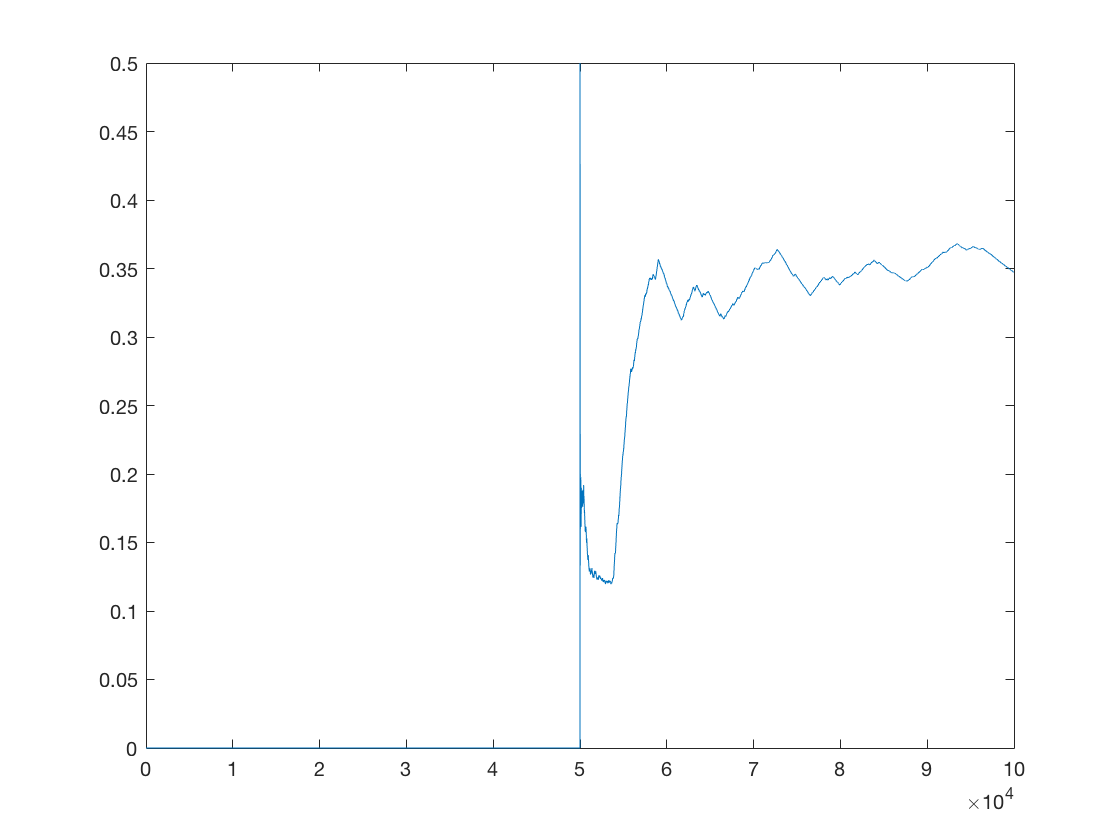
\includegraphics[width=\linewidth]{half_half_tau_prob.png}
    \end{minipage}
\end{figure}

\begin{figure}[!htb]
    \begin{minipage}{0.48\textwidth}
        \centering
        \caption{$\tau^{(0)} = 0, \alpha^{(0)} = 1$, $\tau$ average}
        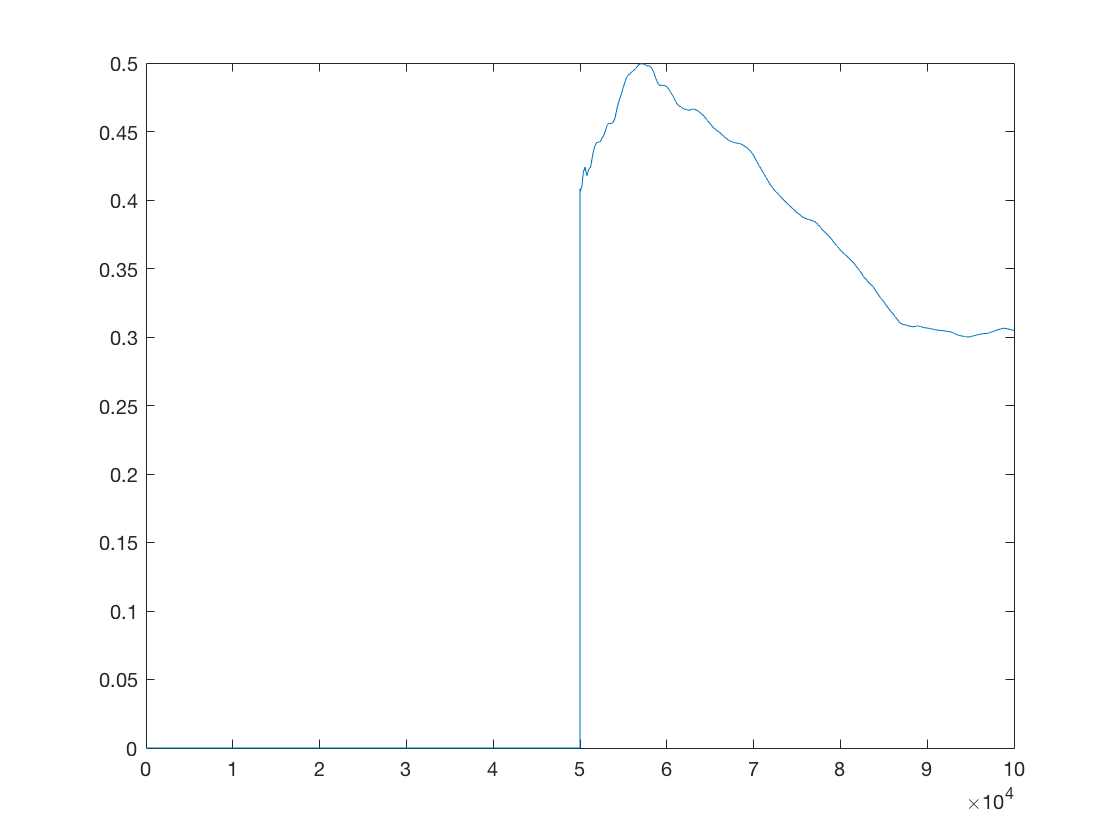
\includegraphics[width=\linewidth]{zero_one_tau_avg.png}
    \end{minipage} \hfill
    \begin{minipage}{0.48\textwidth}
        \centering
        \caption{$\tau^{(0)} = 0.5, \alpha^{(0)} = 0.5$, $\tau$ average}
        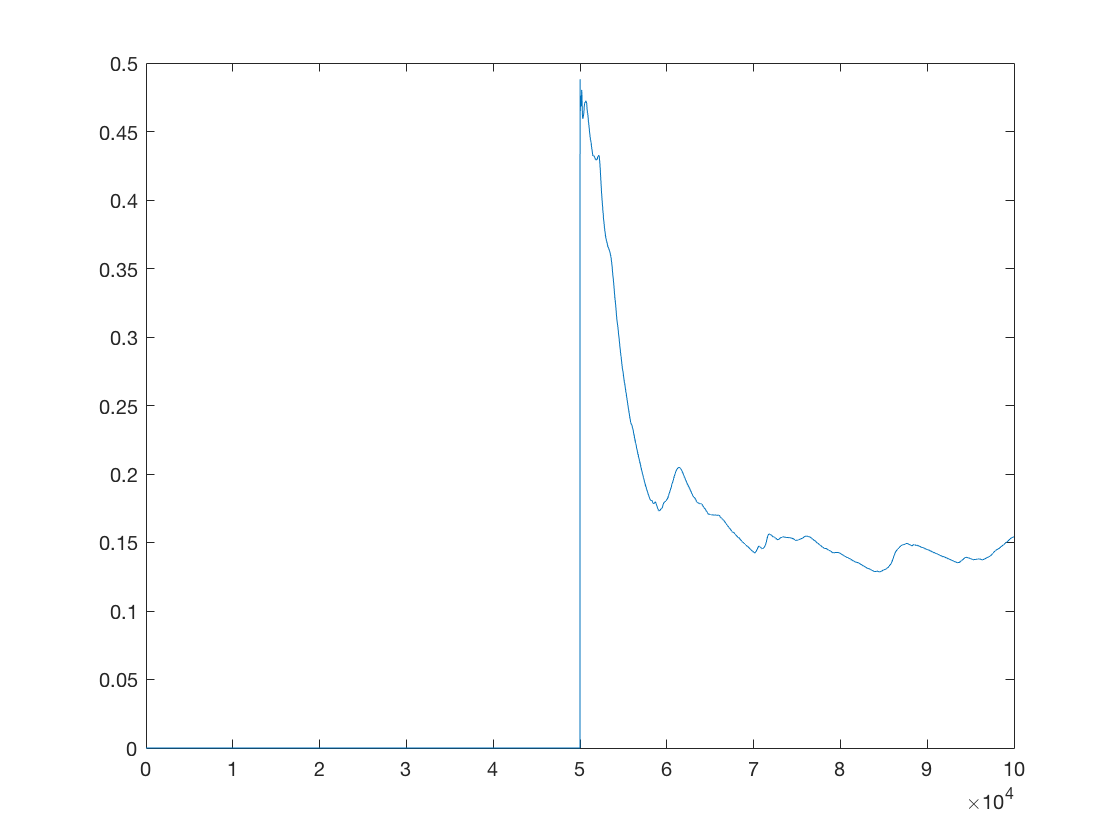
\includegraphics[width=\linewidth]{half_half_tau_avg.png}
    \end{minipage}
\end{figure}

\begin{figure}[!htb]
    \begin{minipage}{0.48\textwidth}
        \centering
        \caption{$\tau^{(0)} = 0, \alpha^{(0)} = 1$, $\alpha$ acceptance probability.}
        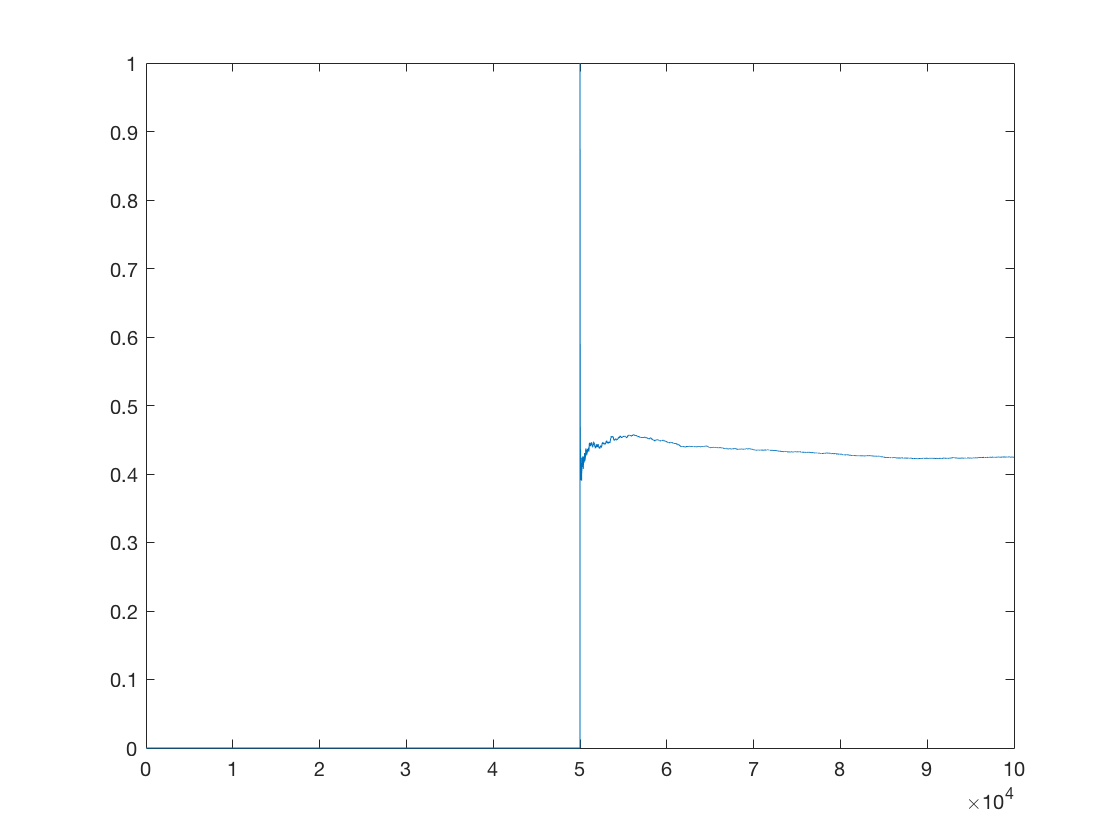
\includegraphics[width=\linewidth]{zero_one_alpha_prob.png}
    \end{minipage} \hfill
    \begin{minipage}{0.48\textwidth}
        \centering
        \caption{$\tau^{(0)} = 0.5, \alpha^{(0)} = 0.5$, $\alpha$ acceptance probability.}
        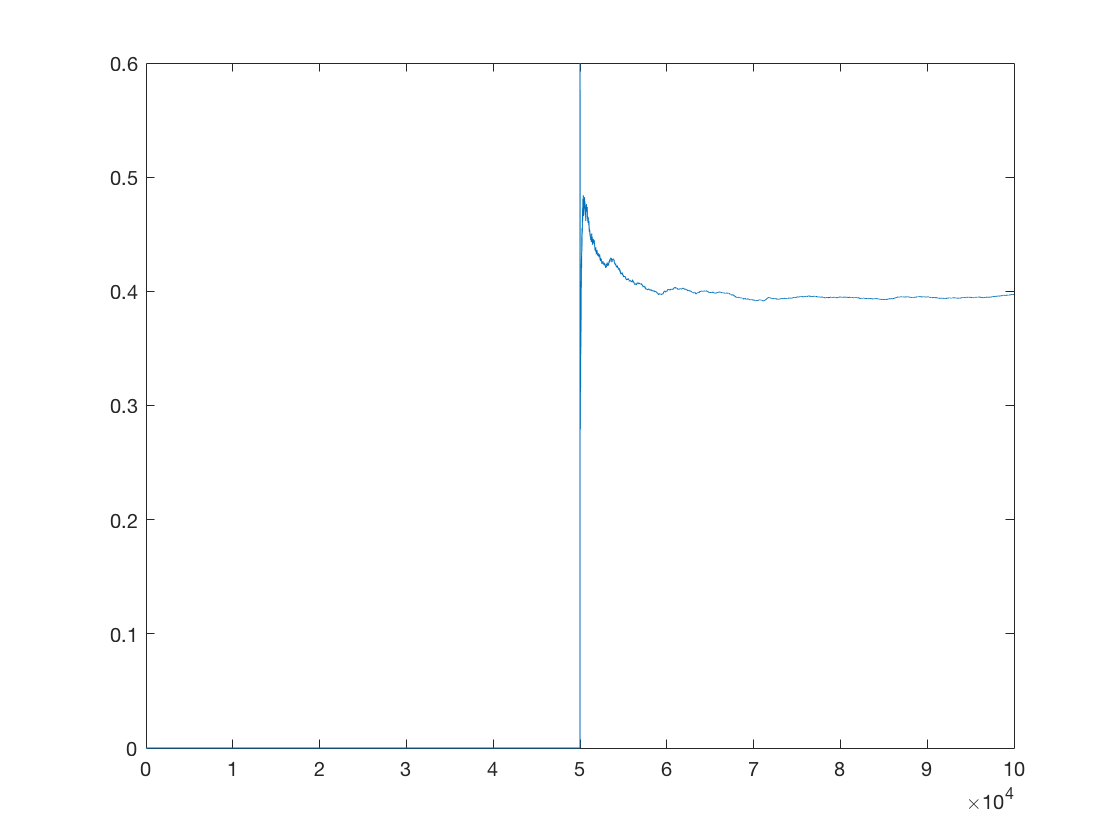
\includegraphics[width=\linewidth]{half_half_alpha_prob.png}
    \end{minipage}
\end{figure}

\begin{figure}[!htb]
    \begin{minipage}{0.48\textwidth}
        \centering
        \caption{$\tau^{(0)} = 0, \alpha^{(0)} = 1$, $\alpha$ average}
        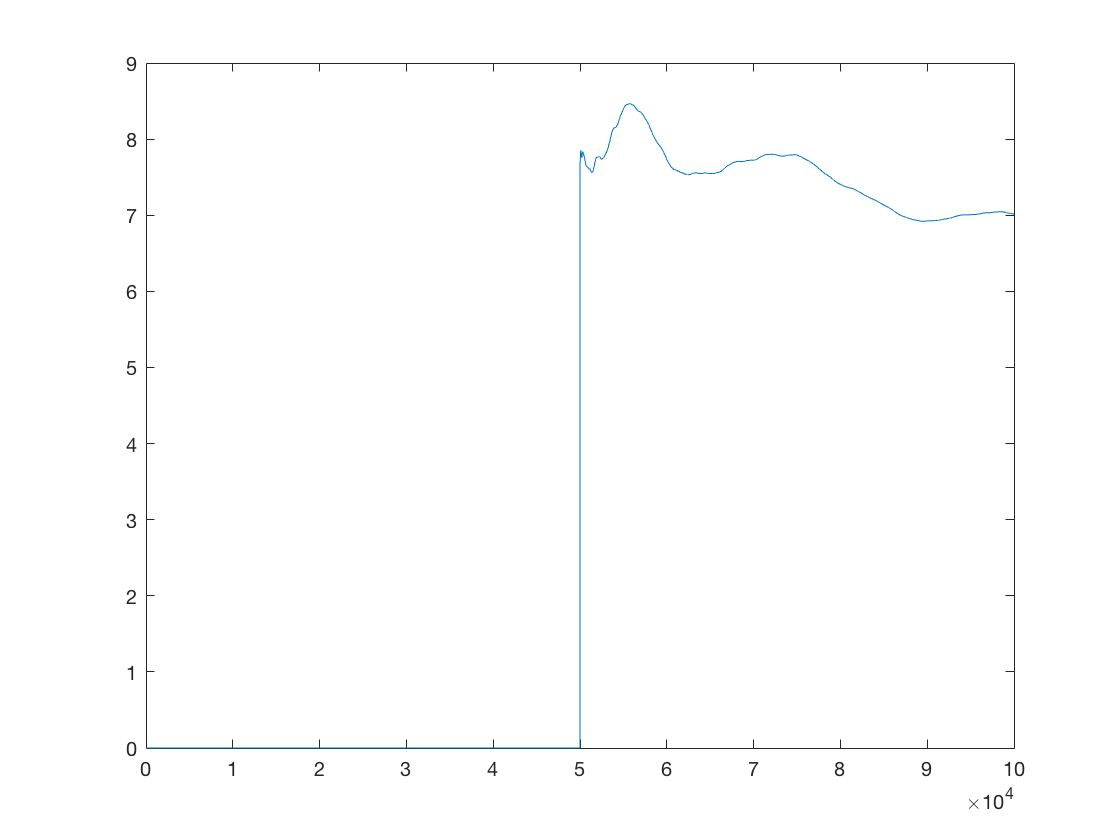
\includegraphics[width=\linewidth]{zero_one_alpha_avg.png}
    \end{minipage} \hfill
    \begin{minipage}{0.48\textwidth}
        \centering
        \caption{$\tau^{(0)} = 0.5, \alpha^{(0)} = 0.5$, $\alpha$ average}
        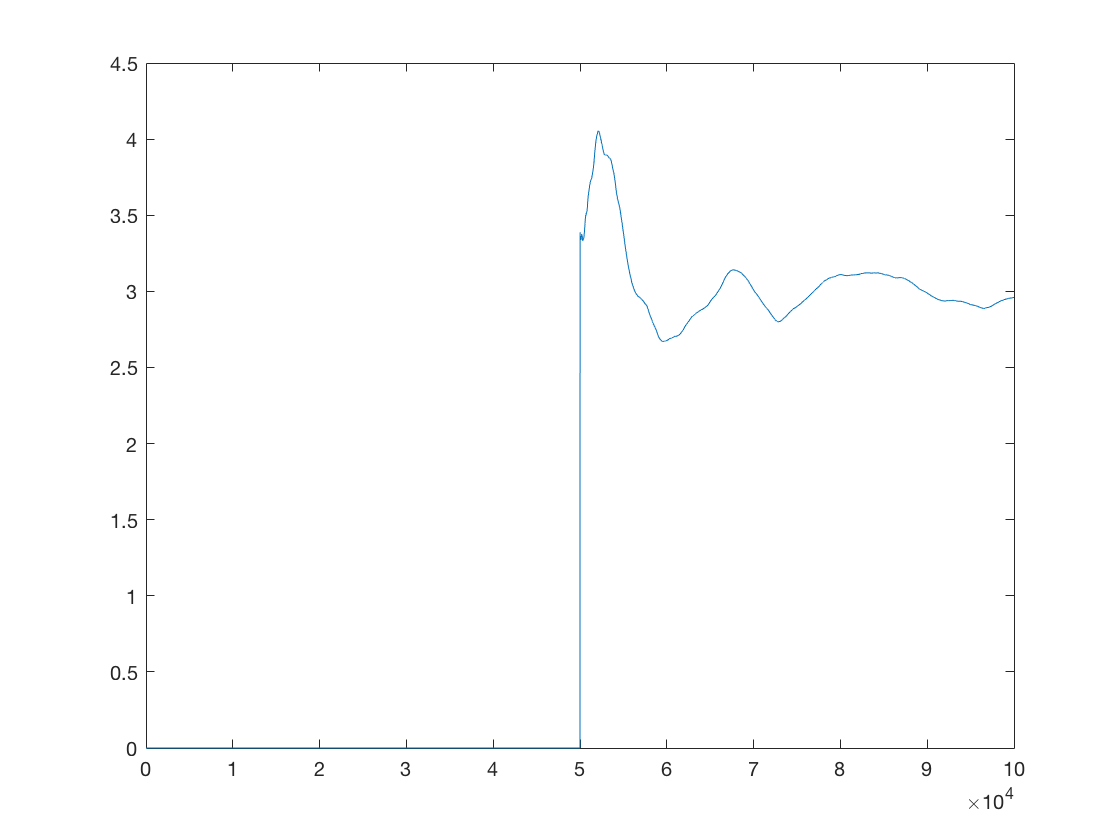
\includegraphics[width=\linewidth]{half_half_alpha_avg.png}
    \end{minipage}
\end{figure}

\end{document}